\chapter{Os Ritos de Passagem}


\begin{center}
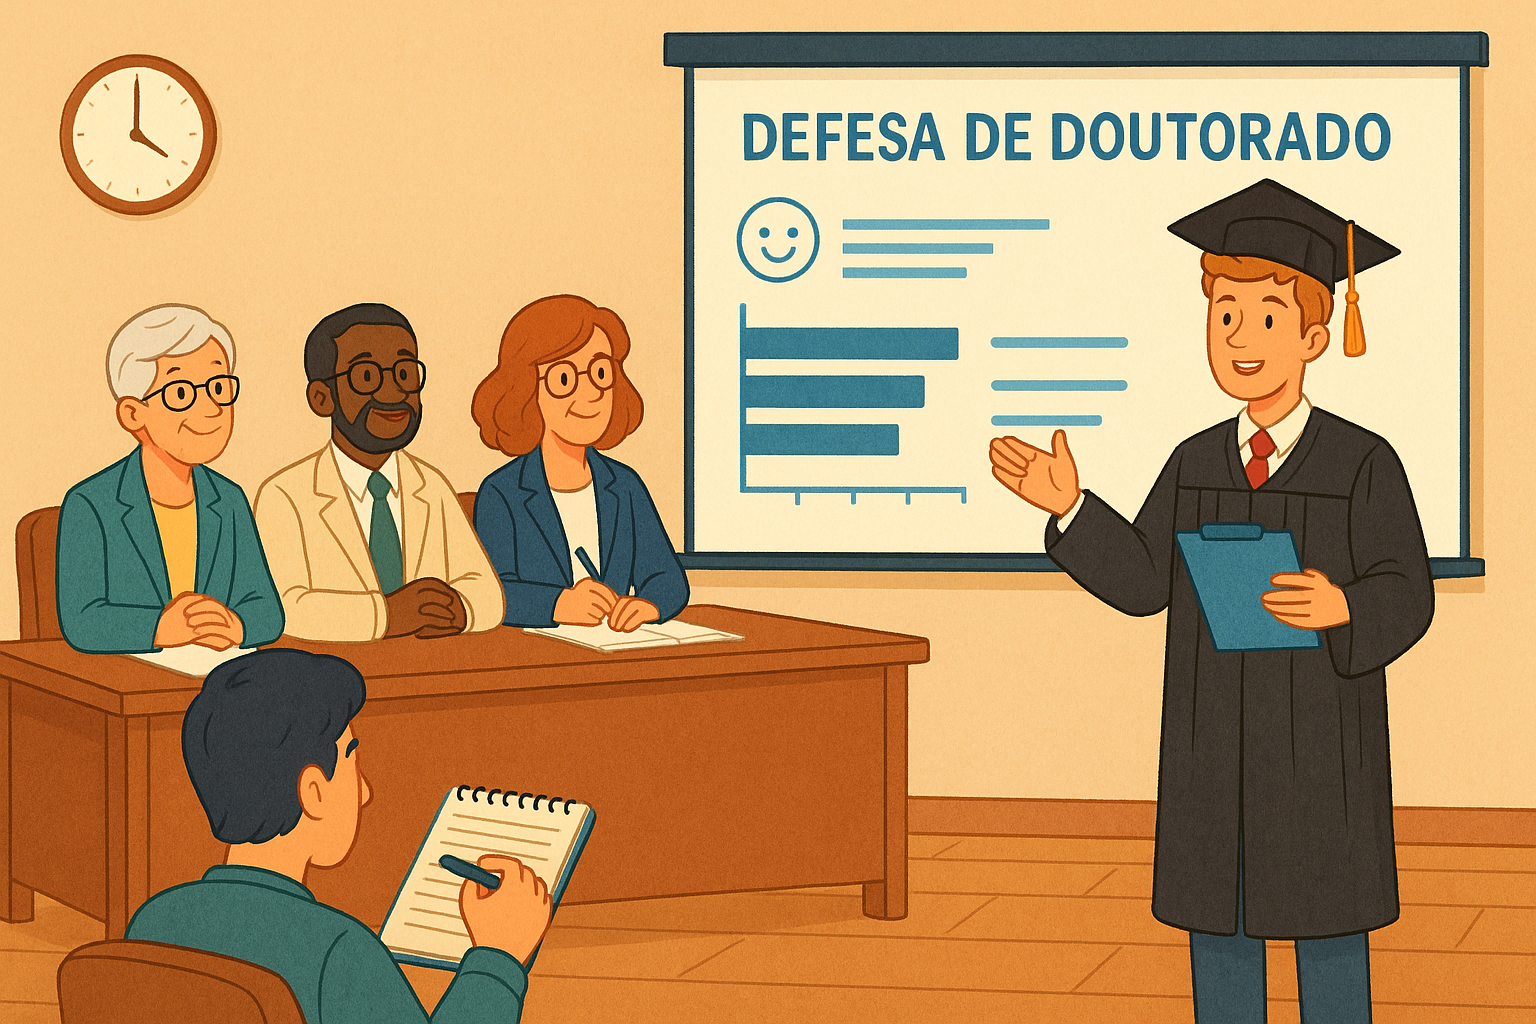
\includegraphics[width=0.5\linewidth]{Images/ritos.png}    
\end{center}
\vspace{0.5cm}

Existem dois importantes ritos de passagem no processo de obter o seu título: a qualificação e a defesa de tese. Normalmente, o aluno passa a ser considerado candidato ao título apenas após um exame de qualificação. 

Praticamente em todos os programas de doutorado, o aluno deve ser aprovado em um exame de qualificação para se tornar um candidato ao doutorado. Já no mestrado, essa obrigação é menos presente\footnote{Para saber mais sobre como as coisas acontecem no PESC/Coppe, veja o \autoref{app:coppedef}}.

\section{O Exame de Qualificação}

O exame de qualificação normalmente busca avaliar 3 quesitos:

\begin{enumerate}
\item	O aluno tem conhecimento suficiente para realizar o doutorado?
\item	O tema de tese conterá uma contribuição original?
\item	O tema de tese é factível?
\end{enumerate}

O momento desse exame varia de programa para programa, e mesmo dentro de um programa, entre os orientadores e alunos. Normalmente, espera-se que se passe um prazo mínimo entre o fim das cadeiras e a realização do exame, para que o aluno tenha um tempo para pesquisar e desenvolver seu tema. 

Em alguns programas, esse exame é feito cedo, tendo mais uma característica de proposta, com muitas suposições. Em outros, ele é feito bem tarde, com o aluno já tendo a tese quase pronta. Esse momento define também o tom do exame.

Um exame mais cedo tem um tom de proposta, e leva muitas vezes a várias discussões, do candidato e da banca, para onde a tese deve se direcionar, que oportunidades são mais claras, e que teorias e métodos podem ser usados. Apesar de eu usar aqui a palavra discussão, deve ser visto como uma discussão colaborativa, onde a banca busca ajudar o futuro candidato. 

Nesse caso, um cuidado a ser tomado é não pensar que o exame de qualificação é como uma tese. Como documento, ele deve ser bem menor; como assunto, ele deve ser focado na proposição e na avaliação de viabilidade. 

Um exame mais tardio tem um tom de pré-defesa, onde a banca já está olhando de forma mais crítica e faz pedidos específicos e orientações mais precisas do que deve ser feito pelo aluno para que ele seja aprovado.

Há locais onde, para o exame ser feito, a tese já tem que estar toda estabelecida e só estejam faltando coisas como partes do experimento final comprobatório ou mesmo uma redação final, funcionando praticamente como um sinal verde para a defesa, ou um sinal de que falta algo importante. 

Para mim, um exame de qualificação de doutorado deve ter pelo menos uma tentativa de solucionar o problema, ou uma investigação na dificuldade de fazê-lo, por meio de tentativas mais ou menos sofisticadas, dependendo do tempo que já foi gasto do prazo da tese.

\subsection{Um Exame para Favorecer o Candidato}

Uma característica do evento de qualificação, seja ele o seminário ou exame, é que a banca é vista como um órgão consultor, ou seja, espera-se que os membros da banca deem sugestões para que o produto final seja melhor. Espera-se que os membros dessa banca participem, mais tarde, da defesa da tese.

Além disso, a banca pode indicar limites, tanto mínimos quanto máximos do que espera da tese ou dissertação. É mais comum que a proposta seja muito ampla, e é costume da banca avisar ao candidato para estreitar seu foco. Raras vezes a banca espera que seja feito mais do que é proposto, mas também é comum que a banca indique caminhos alternativos, ou caminhos adicionais que o candidato pode ou deve seguir, por exemplo, chamando a atenção para um artigo, método ou teoria que o candidato não demonstrou ter conhecimento.

Em todo caso, se espera que esse exame seja para ajudar o candidato, e que, mantendo um padrão de qualidade, permita o que se espera dele na defesa.

\section{A Defesa de Mestrado e Doutorado}

Uma defesa de tese é uma \textbf{apresentação formal} da mesma, na forma de um seminário, pelo candidato, a uma banca de doutores.

Esses doutores são propostos pelo orientador, normalmente, mas não necessariamente, em acordo com o orientado, a um órgão colegiado\footnote{Na Coppe, a CPGP}, que aprova, ou não, a escolha. O orientador escolhe os membros da banca conforme o tema, a experiência e o reconhecimento dos professores convidados, e questões de logística, como disponibilidade nas datas previstas, disponibilidade de verba, etc.

Dependendo do programa, a defesa pode ser realizada na forma presencial, remota ou híbrida. Após a pandemia, e também por dificuldades de verba para viagem de professores, as formas remota e híbrida passaram a ser muito mais aceitas entre os programas.

O candidato deve entregar a sua tese  à banca alguns dias antes, porém esse prazo pode ser menor ou maior de acordo com as circunstâncias e o regulamento\footnote{Na Coppe, o prazo mínimo é 15 dias}. 


\section{Como as Coisas Acontecem na Defesa}

Nesta seção se faz uma narrativa do processo específico da defesa.

\begin{enumerate}
    \item O presidente da banca anuncia o início da defesa, indicando o candidato, o nome da tese, o orientador (normalmente o próprio presidente da banca), a banca (agradecendo a presença) e passa a palavra ao candidato;
    \item O candidato faz a apresentação, na forma de uma palestra de 40 a 50 minutos, onde não pode ser interrompido;
    \item O presidente inicia o processo de comentários e arguição, passando a palavra ao primeiro membro a falar, normalmente ordenando do membro mais externo para o mais interno, sendo os orientadores os últimos a falar;
    \item em sua vez de falar, os membros da banca podem, ou não, fazer perguntas para ser respondidas imediatamente, ou no final de sua fala, ao candidato;
    \item após os membros da banca comentarem a dissertação ou questionarem os candidatos sobre a mesma, a palavra é passada a plateia, que pode ou não se manifestar (normalmente não se manifesta);
    \item o candidato e a plateia se retiram da sala para a banca deliberar (ou banca se retira, principalmente em defesas virtuais);
    \item a banca convoca o candidato e plateia para ler o resultado;
    \item o resultado é lido;
    \item a ata é assinada e se encerra a defesa.
\end{enumerate}

%\needspace{5\baselineskip}
\section{Comportamento e Preocupações do Candidato}

Você deve se preparar para a defesa. No caso de defesa em sala de aula, você deve chegar mais cedo (talvez ir alguns dias antes) para ver como é a sala. 

Deve levar seu próprio computador, um pen-drive de reserva com a apresentação. Não conte com a internet funcionando (Google Slides, por exemplo). Não conte com um computador a sua disposição (apesar de normalmente haver um). 

No caso de defesa remota, você deve ter como fazer a defesa de ``qualquer maneira'', para isso:
\begin{itemize}
    \item Tenha um acesso de internet alternativo. Celulares, por exemplo, podem ser ligados a um computador via USB para funcionarem como modem, ou podem oferecer uma rede wi-fi com a funcionalidade de ``tethering''.
    \item Tenha um computador reserva, pois a casos que o computador dá problema
    \item Verifique antes se câmera, microfone e fone estão funcionando. É essencial que a defesa possua a câmera.
    \item Prepare o celular para backup de câmera, fone e microfone.
    \item Tenha um lugar reserva, pois já aconteceu de ser necessário por falta de luz, internet, etc. 
\end{itemize}

Alguns orientadores fazem uma apresentação prévia\footnote{Não é o meu caso}, outros discutem os slides\footnote{Eu posso rever algumas vezes}. Pergunte o que seu orientador deseja.



\subsection{Slides}

Veja as dicas em \expurl{https://github.com/xexeo/DicasSlidesAcademicos/blob/main/DicasSlidesAcademicos.pdf}{Dicas de Slides Acadêmicos}.

Em especial:
\begin{itemize}
    \item Cuidado com ortografia e gramática;
    \item Cuidado com o tamanho de imagens, principalmente nas letras das imagens, para que sejam legíveis;
    \item Numere os slides, e coloque o total de slides;
    \item Não encha os slides de texto;
    \item Não use corpo de fonte menor que 16;
    \item Tente usar corpo 30;
    \item Não faça show de efeitos especiais, mas use se necessário;
    \item Não se esqueça de dar a atribuição de todas as imagens;
    \item Não se esquecer de agradecer os órgãos financiadores, e
    \item Use as logomarcas institucionais.
\end{itemize}

\subsection{Ao apresentar}

Não fique de costas para a banca lendo os slides. Sua apresentação deve ser de frente para a banca e a plateia, sabendo o que vai falar, por isso deve treinar. Não precisa saber de cor. A \autoref{fig:comparacao-apresentacoes} ilustra esse assunto. 

Nem para apontar para o slide fique de costas para a banca, no máximo fique de lado. Olhe para todos na plateia ao longo da apresentação.

Se preciso, faça anotações sobre o que deve falar, mas não para ler as anotações, mas de forma que elas possam guiá-lo. Os slides devem funcionar da mesma forma.

\begin{figure}[hbt]
    \centering
    \begin{subfigure}[b]{0.45\textwidth}
        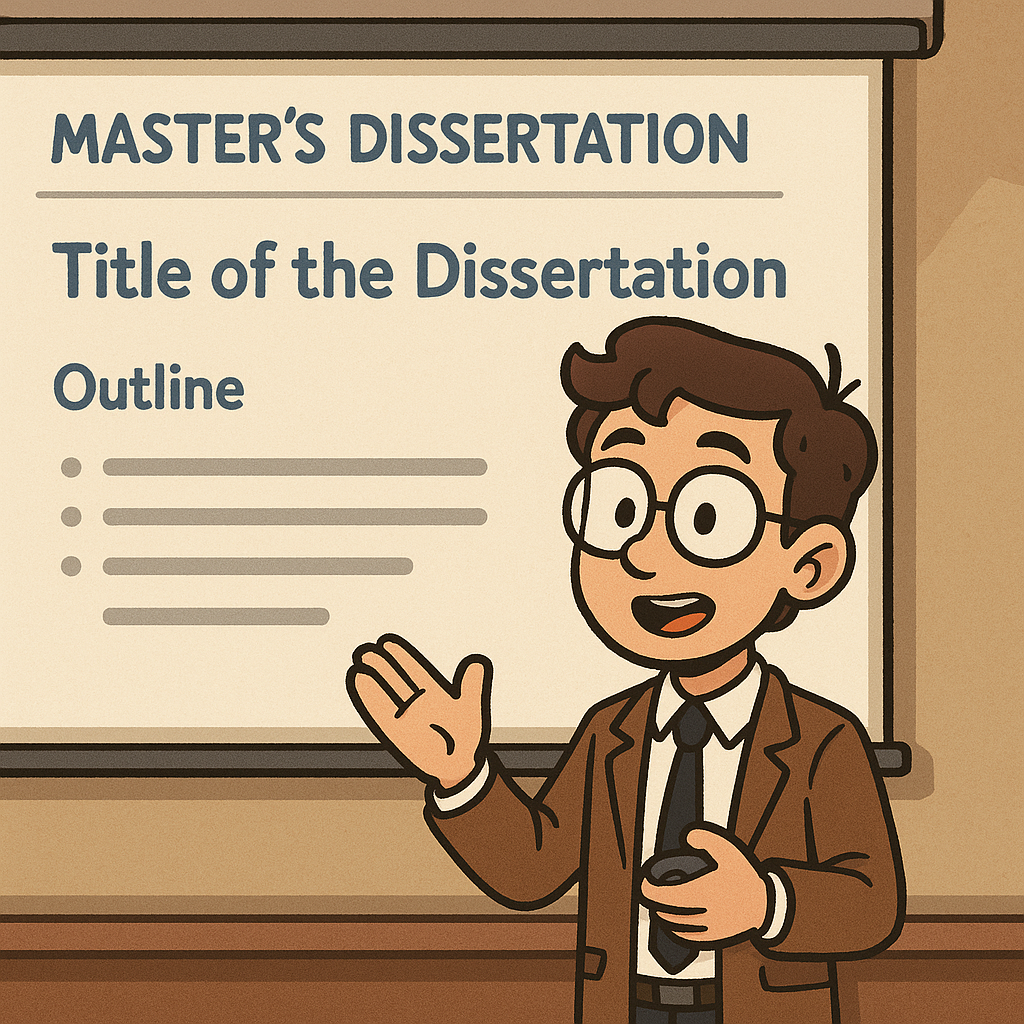
\includegraphics[width=\linewidth]{Images/dandoaulacerto.png}
        \caption{Posicionamento correto do candidato.}
        \label{fig:apresentacao-correta}
    \end{subfigure}
    \hfill
    \begin{subfigure}[b]{0.45\textwidth}
        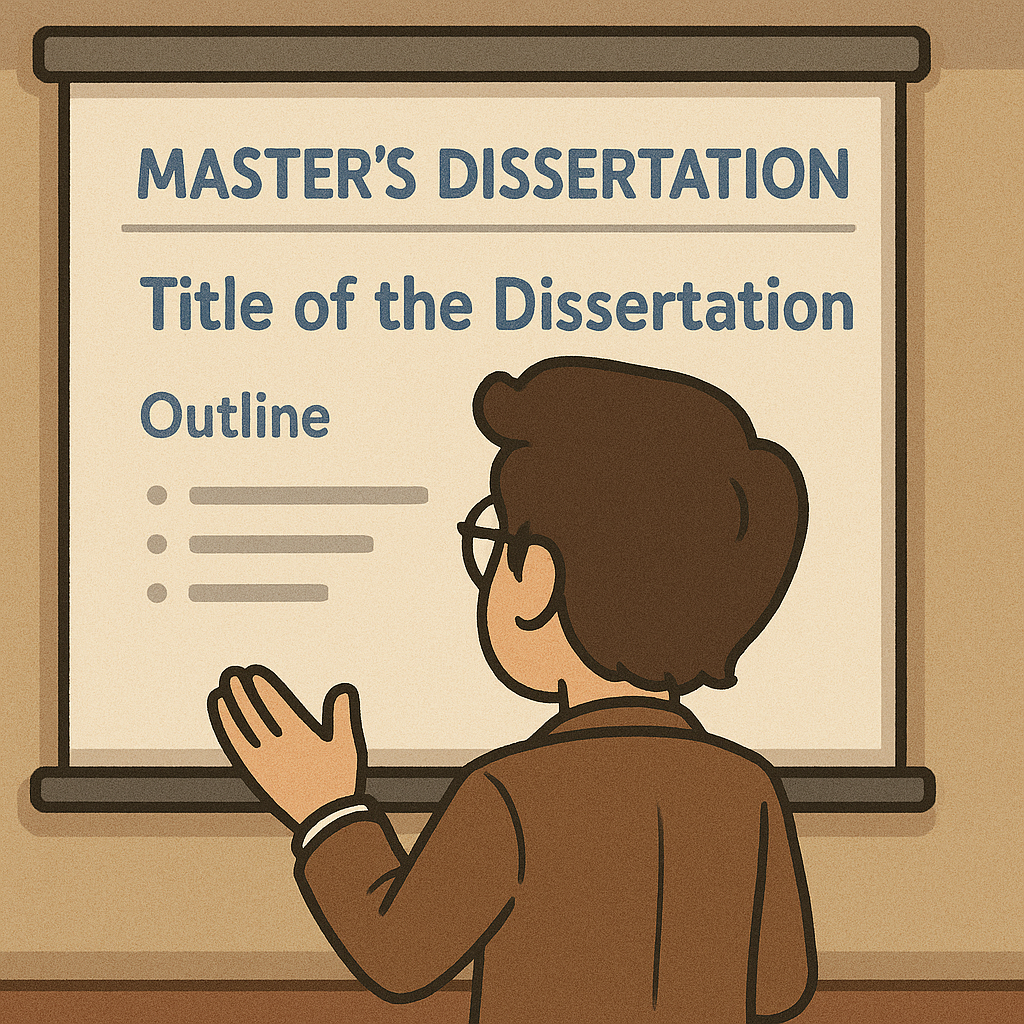
\includegraphics[width=\linewidth]{Images/dandoaulaerrado.png}
        \caption{Posicionamento indevido do candidato.}
        \label{fig:erro-apresentacao}
    \end{subfigure}
    \caption{Comparação entre uma apresentação correta e uma com erro.}
    \label{fig:comparacao-apresentacoes}
\end{figure}



\subsection{Demonstrações de Software}

A melhor forma de demonstrar software é por meio de gravações do sistema funcionando e não rodar diretamente. A experiência prova que é comum que aconteçam problemas de última hora que devem ser evitados. Grave uma utilização e de preferência faça cortes que reduzam os tempos de espera, digitação, etc...

\subsection{Para ficar mais calmo}

É normal ficar nervoso, mas há formas de ajudar a acalmar.
\begin{itemize}
    \item Treine antes, principalmente para fazer a apresentação no tempo. Se você está treinado, vai ficar mais calmo, porque sabe o que tem que fazer.
    \item Tenha com você um copo/garrafa de água, se ficar nervoso, se perder, ou algo assim, pare, respire, tome um gole de água, veja em que ponto está, e então continue com mais calma. O copo de água está ali tanto para matar a sede, como para servir de intervalo sem causar polêmica.
    \item Pelo menos uma vez, no treinamento, grave e veja você apresentando e tente corrigir depois os maus hábitos.
\end{itemize}

\subsection{Durante as perguntas e comentários}

\textbf{Você deve anotar} os que os membros da banca falam. Para isso leve um caderno e caneta. Se quiser gravar (não deixando de anotar), deve pedir autorização. Não anotar é até uma falta de respeito aos comentários da banca. Não é para copiar todas as falas, mas sim deixar um guia para você responder, seja na hora, seja nas correções da dissertação.

Mesmo que o membro da banca fale ``Não precisa anotar porque eu coloquei tudo na dissertação'' ou ``Eu vou te mandar tudo'', anotar é importante para entender o que o membro da banca acha importante, e que perguntas foram feitas.

\section{Os Resultados}

Normalmente os programas admitem três resultados possíveis:
\begin{itemize}
    \item \textbf{Aprovação da dissertação por unanimidade}: significa que você foi aprovado sem modificações de relevância. A banca, e a instituição, ainda esperam que algumas modificações sugeridas sejam feitas, e o aluno tem 30 dias para depositar a versão final no registro e no PESC. O orientador pode ou não auxiliar nas modificações, dependendo da importância delas.
    \item \textbf{Aprovação  somente  após  satisfazer  as  exigências que constam 	 na  folha  de   modificações  no  prazo   fixado  pela  banca    ( não superior  a   uma quantidade de  dias)}: nesse caso, que é comum, será criada uma ata adicional com uma lista de mudanças, e haverá um ou dois indicados para verificar as modificações foram feitas. Normalmente isso significa que a banca reconhece que foi feito um trabalho que quase atingiu o nível necessário do mestrado, mas que precisa de esforços adicionais, ou que precisa de grandes correções de texto. Algumas vezes isso é usado como uma última chance ao candidato e as modificações são de grande monta, podendo resultar na reprovação. Outras vezes é usado como uma forma de garantir um prazo hábil para o candidato fazer mudanças de grande monta no texto, mas considerando que sua aprovação é muito provável.
    \item \textbf{Reprovação da dissertação}: uma ocorrência rara, mas possível, e provavelmente indicada anteriormente pelo orientador sobre sua possibilidade. Indica que o aluno não atingiu o mínimo desejável para o bter o título de mestrado. Já vi algumas reprovações, sendo que os motivos incluíram plágio, experiências não realizadas, e baixa qualidade total do trabalho que tinha sido avisada pelo orientador.
\end{itemize}

Normalmente a reprovação é final, porém eu conheço pelo menos um programa que permite uma nova defesa em um prazo máximo de 6 meses.


